\documentclass[../main]{subfiles}

\begin{document}
\section{Hoja de ruta}

\subsection{Configuración de Hardware}

\setcounter{subsubsection}{-1}

\subsubsection{Recursos a usar}

\begin{itemize}
	\item ESP32: Controlador principal con conectividad Wi-Fi.
	\item Sensor BME280: Sensor para medir temperatura, humedad y presión.
	\item Sensor MQ135: Sensor para la detección de la concentración de CO2 en el aire.
	\item Sensor de Humedad de Suelo: Sensor analógico para medir el nivel de humedad del suelo.
	\item Protoboard y Jumpers: Para facilitar las conexiones de prueba.
	\item Fuente de Alimentación: Batería o adaptador USB de 5V.
	\item Cables Dupont: Para realizar las conexiones entre los sensores y el ESP32.
\end{itemize}

\subsubsection{Diagrama de Conexiones}

\begin{itemize}
	\item ESP32: Este será el controlador principal y estará encargado de leer los datos de cada sensor.
	\item BME280: Este sensor utiliza la comunicación I2C para conectarse con el ESP32. Las conexiones necesarias son:
	      \begin{enumerate}
		      \item VCC a \qty{3.3}{\V} del ESP32.
		      \item GND a GND del ESP32.
		      \item SCL al pin D22 del ESP32.
		      \item SDA al pin D21 del ESP32.
	      \end{enumerate}
	\item MQ135: Para el sensor MQ135, se utilizará la salida analógica para la detección de CO2.
	      \begin{enumerate}
		      \item VCC a \qty{5}{\V} del ESP32.
		      \item GND a GND del ESP32.
		      \item AOUT a un pin analógico del ESP32.
	      \end{enumerate}
	\item Sensor de Humedad de Suelo: El sensor de humedad de suelo puede ser analógico o digital. Se optará por la salida analógica para una medición más precisa.
	      \begin{enumerate}
		      \item VCC a \qty{3.3}{\V} del ESP32.
		      \item GND a GND del ESP32.
		      \item AOUT a un pin analógico del ESP32.
	      \end{enumerate}
\end{itemize}

\subsubsection{Soporte del ESP32 en Arduino IDE}

Para poder programar en ESP32 con Arduino, es necesario agregar un URL en el
gestor de placas lo siguiente:
\url{https://dl.espressif.com/dl/package_esp32_index.json}

\begin{figure}[H]
	\centering
	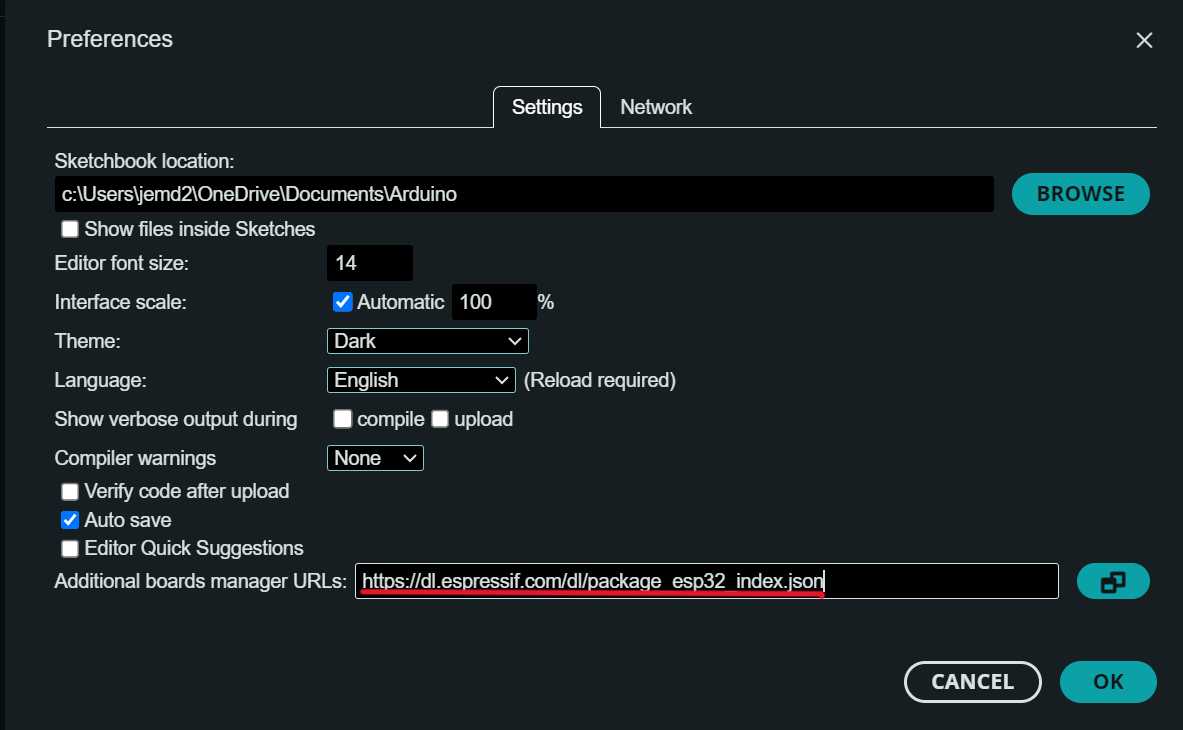
\includegraphics[width = 13cm]{res/configuracionParaEsp32.png}
\end{figure}

\subsubsection{Conexión con Firebase}

Para realizar una conexión a Firebase desde tu ESP32, es utilizada la biblioteca
Firebase ESP32 Client.

\subsection{Programación de aplicación}

\setcounter{subsubsection}{-1}

\subsubsection{Recursos a usar}

\begin{itemize}
	\item Kotlin: lenguaje principal de desarrollo
	      \footnote{\url{https://kotlinlang.org/}}
	\item Firebase Realtime Database: almacenamiento de observaciones y perfiles
	      \footnote{\url{https://firebase.google.com/}}
	\item Androidplot: biblioteca para la creación de gráficos
	      \footnote{\url{https://github.com/halfhp/androidplot}}
\end{itemize}


\subsubsection{Estructura de la aplicación}
La aplicación está estructurada 4 actividades principales:
\begin{itemize}
	\item Actividad de visualización de datos y gráficas (MainActivity) : Se muestran los datos recibidos por la placa y su interpretación respecto al perfil elegido por el usuario.
	\item Actividad de elección de perfiles (ProfileActivity) : Se muestran todos los perfiles disponibles para su selección en \textbf{MainActivity}.
	\item Actividad de modificación de perfiles (DisplayProfileActivity): Se muestra todos los datos del perfil seleccionado, así como la opción de modificarlo o eliminarlo.
	\item Actividad de creación de perfiles (NewProfileActivity): Se muestra un campo para poder crear un nuevo perfil existente.
\end{itemize}
En la aplicación, se han usado dos estructuras de datos para abstraer los datos de los sensores y de los perfiles\\
\textbf{Clase Profile}
\begin{lstlisting}[language = Kotlin]
	package com.mypackage.espapplication.models

	import android.os.Parcelable
	import kotlinx.parcelize.Parcelize

	@Parcelize
	data class Parameter(
    	var maxValue : Double = 0.0,
    	var minValue : Double = 0.0
	) : Parcelable

	@Parcelize
	data class Profile(
		var id : String? = null,
		var name : String = "defaultProfile",
		var alcohol : Parameter = Parameter(),
		var altitud : Parameter = Parameter(),
		var co2 : Parameter = Parameter(),
		var humedaddesuelo : Parameter = Parameter(),
		var presion : Parameter = Parameter(),
		var temperatura : Parameter = Parameter()) : Parcelable
\end{lstlisting}
\textbf{Clase SensorValues}
\begin{lstlisting}[language=Kotlin]
	package com.mypackage.espapplication.models

	class SensorValues (
		val alcohol : Double = 0.0,
		val altitud : Double = 0.0,
		val co2 : Double = 0.0,
		val estado : Int = 1,
		val humedaddesuelo : Double = 0.0,
		val presion : Double = 0.0,
		val temperatura : Double = 0.0)
\end{lstlisting}

\newpage
\begin{landscape}
	\begin{figure}[H]
		\centering
		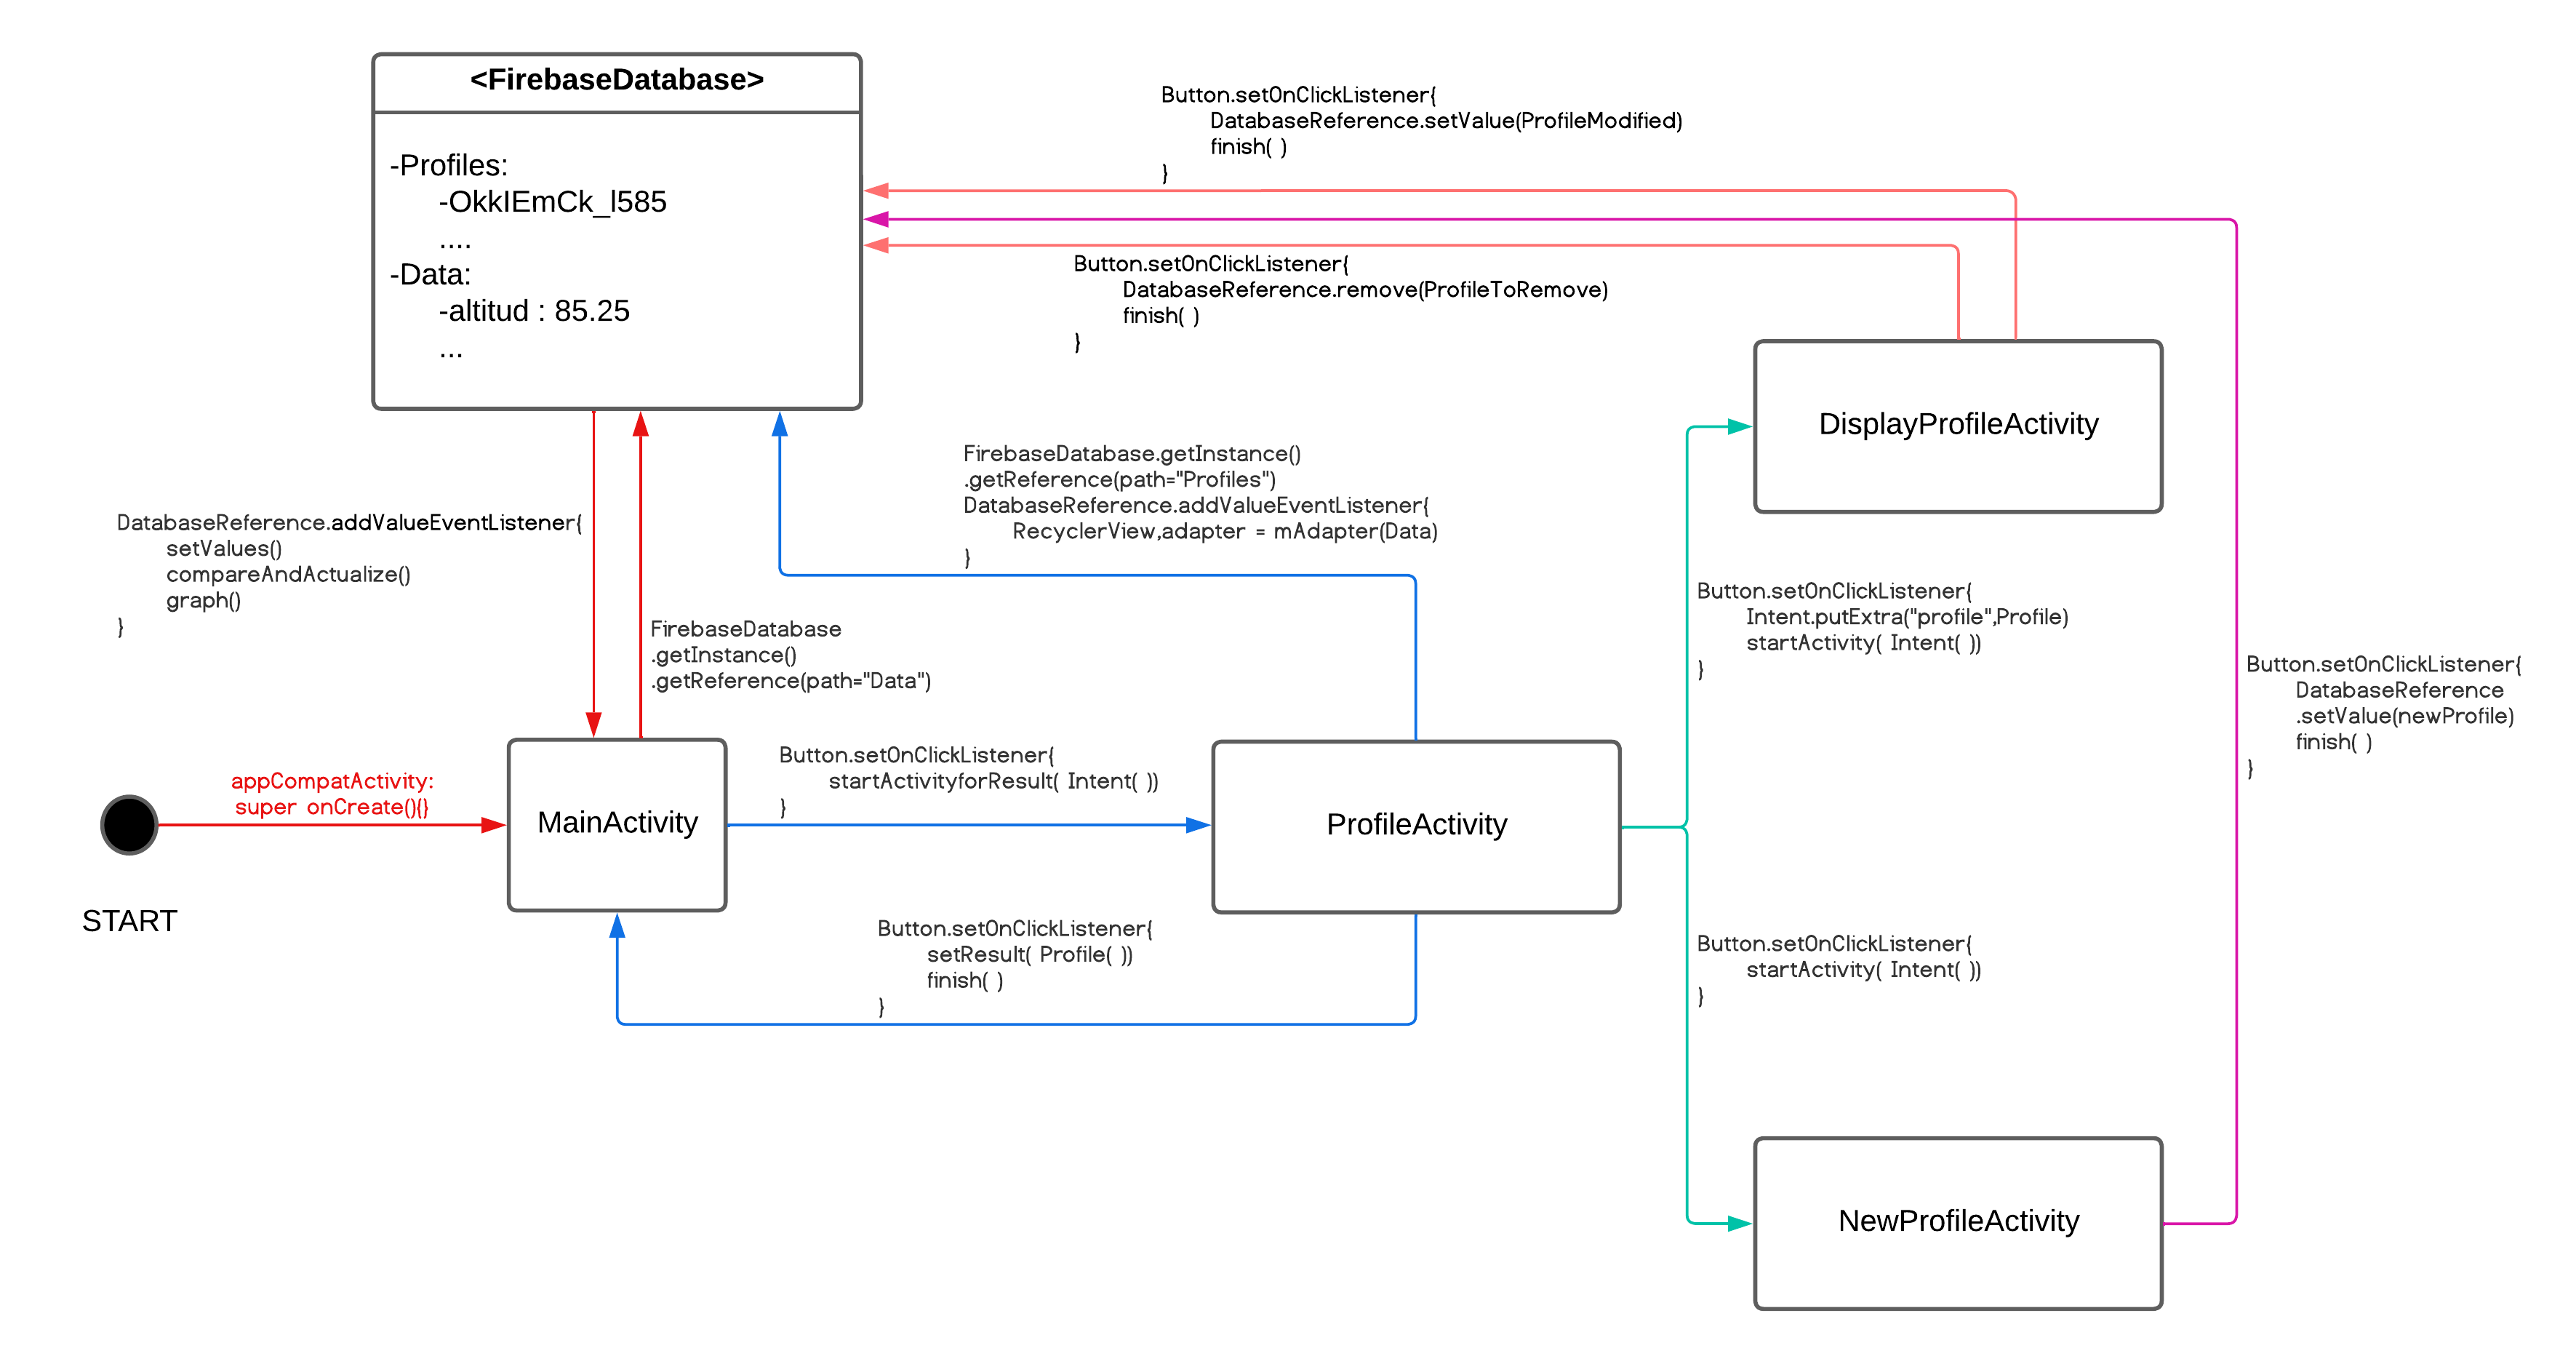
\includegraphics[height=0.86\textheight]{res/appDiagram.png}
		\caption{Diagrama de funcionamiento de la aplicación}
	\end{figure}
\end{landscape}
\newpage

\subsubsection{Visualización de Datos y Gráficos : Gráfica en tiempo real}
La visualización de datos y gráficos se realiza de manera dinámica en la actividad principal de la aplicación.
Los parámetros que se visualizan en la aplicación son:
\begin{itemize}
	\item Alcohol
	\item Altitud
	\item $CO_2$
	\item Humedad
	\item Presión
	\item Temperatura
\end{itemize}
La generación de gráficos se realizará mediante la librería \textit{AndroidPlot}, utilizando un objeto \textit{XYPlot} para visualizar la información enviada por la placa, cada vez que
ésta se conecte a la base de datos.
\begin{figure}[H]
	\centering
	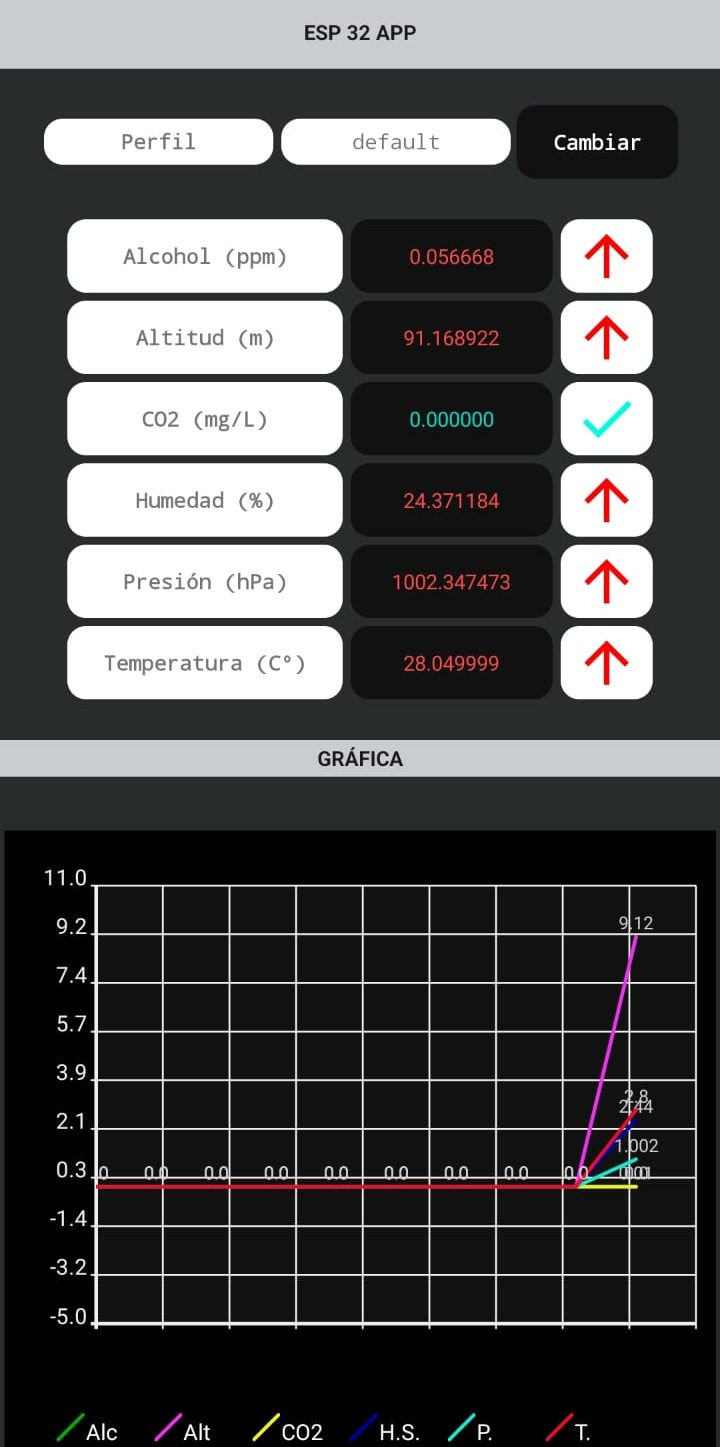
\includegraphics[scale=0.35]{res/uiPreview.jpg}
	\caption{Visualización de parámetros y gráfico en tiempo real}
	\label{FiguraDeGráficos}
\end{figure}
\end{document}
